\documentclass[12pt,letterpaper,titlepage]{report}

%%% packages %%%

\usepackage{geometry}
\usepackage{makecell}
\usepackage{graphicx}

%%% metadata %%%

\graphicspath{{images/}}

\newcommand{\myTitle}{Magnetic Field in a Current-Carrying Coil}
\newcommand{\myName}{Shawn Lutch, SML0262}
\newcommand{\myPeriod}{PHYS 2240.503}

\usepackage[pdftex,
            pdfauthor={\myName{}},
            pdfsubject={\myPeriod{}},
            pdftitle={\myTitle{}},
            pdfproducer={\myName{} via PDFTeX},
            pdfcreator={pdflatex}]{hyperref}    

%%% layout %%%

\pagenumbering{gobble}
\raggedright
\geometry{
    letterpaper,
    lmargin=0.75in,
    rmargin=0.75in,
    tmargin=1in,
    bmargin=1in
}

%%% document below %%%

\begin{document}

%% title page

\title{\myTitle{}}
\author{\myName{} \\ \myPeriod{}}
\date{\today}
\maketitle

%% abstract

\section*{Abstract}

We used a magnetic field sensor to measure the axial and radial components of the magnetic field generated by a current-carrying coil. We calculate that the magnetic field strength of our solenoid is between 22.016 and 26.420 mT. In gathering our data, the magnetic field sensor was not kept exactly in line with the vertical axis of the coil, introducing the radial component of the field vector into our axial field data and causing discrepancies in the data.

%% introduction

\section*{Introduction}

In this lab, we will move a magnetic field sensor through a current-carrying coil and record data about the magnetic field in order to compare changes in axial and radial components of the field. We will attach the magnetic field sensor to a rotary motion sensor in order to record the position of the magnetic field sensor relative to the coil.

\bigskip
When referring to the magnetic field created by a solenoid, we call the component that runs parallel to the vertical axis of the solenoid the \textbf{axial component} of the field; likewise, we call the component that runs perpendicular to the vertical axis of the solenoid the \textbf{radial component} of the field. The direction of each field component, as measured by the sensor, is relative to the orientation of the sensor. This direction is shown with positive and negative values.

\bigskip
The general equation for finding the magnetic field along the perpendicular axis through the center of a coil of wire with negligible length, radius $R$, and $N$ turns of wire (\textbf{Equation \ref{single_coil}}) is

\begin{equation} \label{single_coil}
B = \frac{\mu_0 N I R^2}{2 ( x^2 + R^2 )^{3/2}}
\end{equation}

where \textbf{$\mu_0$} $= 4 \pi \times 10^{-7}$ $T \cdot \frac{m}{A}$ is the permittivity of free space, \textbf{$I$} is the current through the coil, and \textbf{$x$} is the distance from the center of the coil. To find the magnetic field of a long solenoid with $n$ turns per unit length, we use \textbf{Equation \ref{long_solenoid}}:

\begin{equation} \label{long_solenoid}
B = \mu_0 n I
\end{equation}

where $\mu_0$ is again the permittivity of free space, shown above. Equation \ref{long_solenoid} fails when approaching the ends of the solenoid, where the magnetic field strength begins to decrease.

\bigskip
To be considered a \textit{long} solenoid, the length of the coil inside the solenoid must be significantly longer than the diameter of the coil. Solenoids that do not fit this description are referred to as \textit{short} solenoids. For short solenoids, we are not able to use either Equation \ref{single_coil} because the length of the coil is too long, and we are not able to use Equation \ref{long_solenoid} because the length of the coil is too short. Instead, the two equations provide bounds on the value of the magnetic field.

\bigskip
\bigskip
\begin{minipage}{\textwidth}
    \centering
    \begin{tabular}{| l | r |} \hline
    
    $N$  &  600 turns \\ \hline
    $R$  &  0.015 m   \\ \hline
    $L$  &  0.025 m   \\ \hline
    
\end{tabular}
    \\ \medskip
    Specifications for the Coil
\end{minipage}
\pagebreak

%% apparatus

\section*{Apparatus}

\begin{itemize}
    \item AC/DC Electronics Laboratory
    \item Rotary Motion Sensor
    \item 2-Axis Magnetic Field Sensor
    \item Short Patch Cord (x8)
    \item Large Rod Base
    \item 90-cm Rod
    \item Mass and Hanger Set
    \item Thread
    \item 850 Universal Interface
    \item PASCO Capstone
\end{itemize}
\bigskip

%% procedure

\section*{Experimental Procedure}

We first zeroed the magnetic field sensor and the rotary motion sensor without any current running through the solenoid. We ran 5V of DC current through the coil, inserted the magnetic field sensor as far as possible into the coil (while centered about the vertical axis of the coil), and recorded the data from the magnetic sensor probe as we slowly pulled the sensor out of the coil with the handle facing north. We labeled this data set \textbf{Center}. We measured and recorded the peak amplitude.

\bigskip
We repeated this process with the probe held against the \textbf{East} wall of the coil, and again with the probe held against the \textbf{West} wall of the coil. We switched the patch cords, reversing the direction of the current through the coil and repeated the process with the probe held against the east wall of the coil. We labeled this data set \textbf{East, rev}.

\bigskip
We then calculated the bound values for our solenoid using Equations \ref{single_coil} and \ref{long_solenoid}.

\pagebreak

%% data

\section*{Data}

\begin{minipage}{\textwidth}

    \centering
    
    Current through Coil \\
    \medskip
    
    \begin{tabular}{| l | r | r |} \hline
        \thead{Trial} & \thead{Current \\ (A)} & \thead{Axial Peak Ampl. \\ (mT)} \\ \hline
        Center        &  0.876  &   19.154  \\ \hline
        East          &  0.854  &   18.736  \\ \hline
        West          &  0.855  &   19.377  \\ \hline
        East, rev.    &  0.849  & $-18.774$ \\ \hline
    \end{tabular}

\end{minipage}

%% calculations and graphs

\section*{Calculations and Graphs}

\begin{minipage}{\textwidth}
    \centering
    
    \begin{minipage}{.4\textwidth}
        \centering
        Axial Field Graph \\
        
        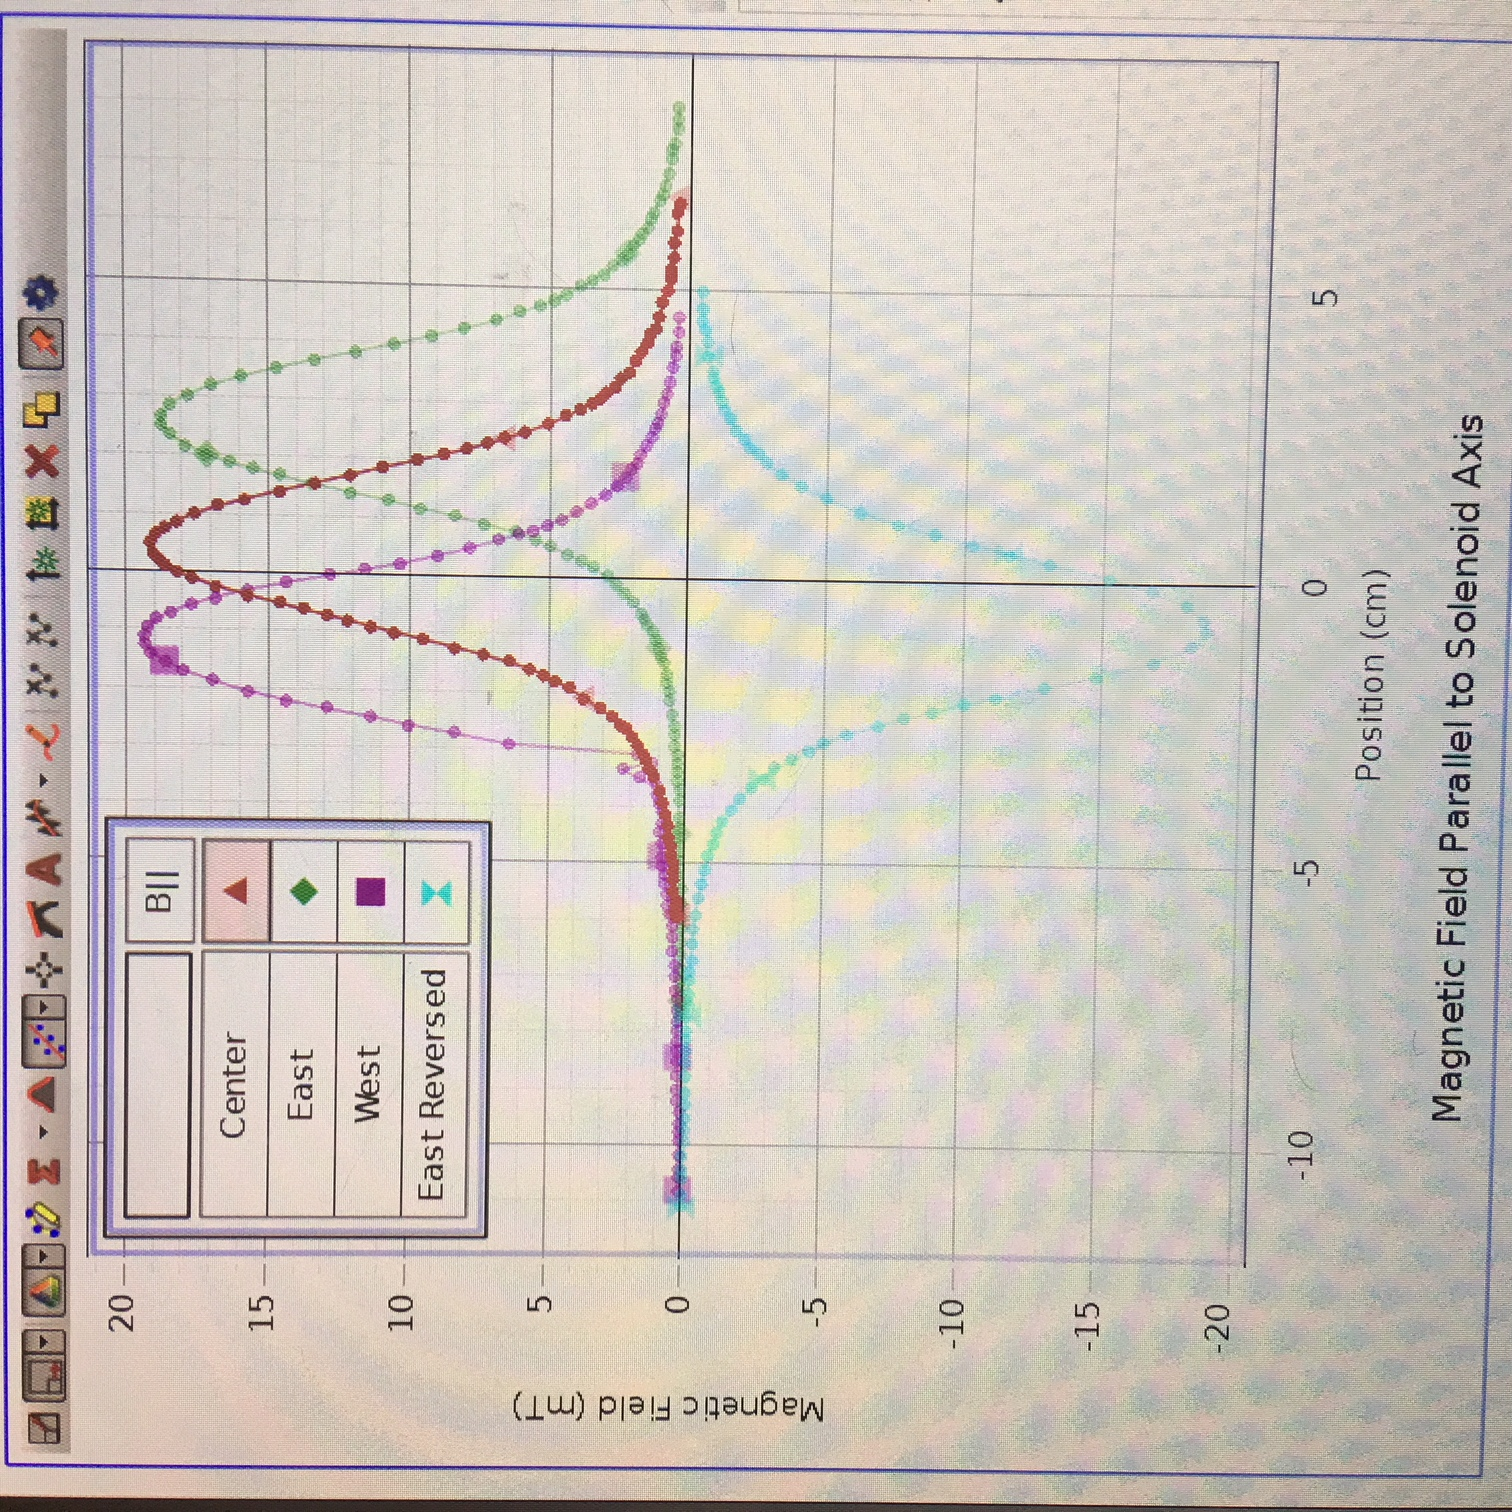
\includegraphics[width=.9\textwidth,angle=270]{axial.jpg}
    \end{minipage}

    \begin{minipage}{.4\textwidth}
        \centering
        Radial Field Graph \\
        
        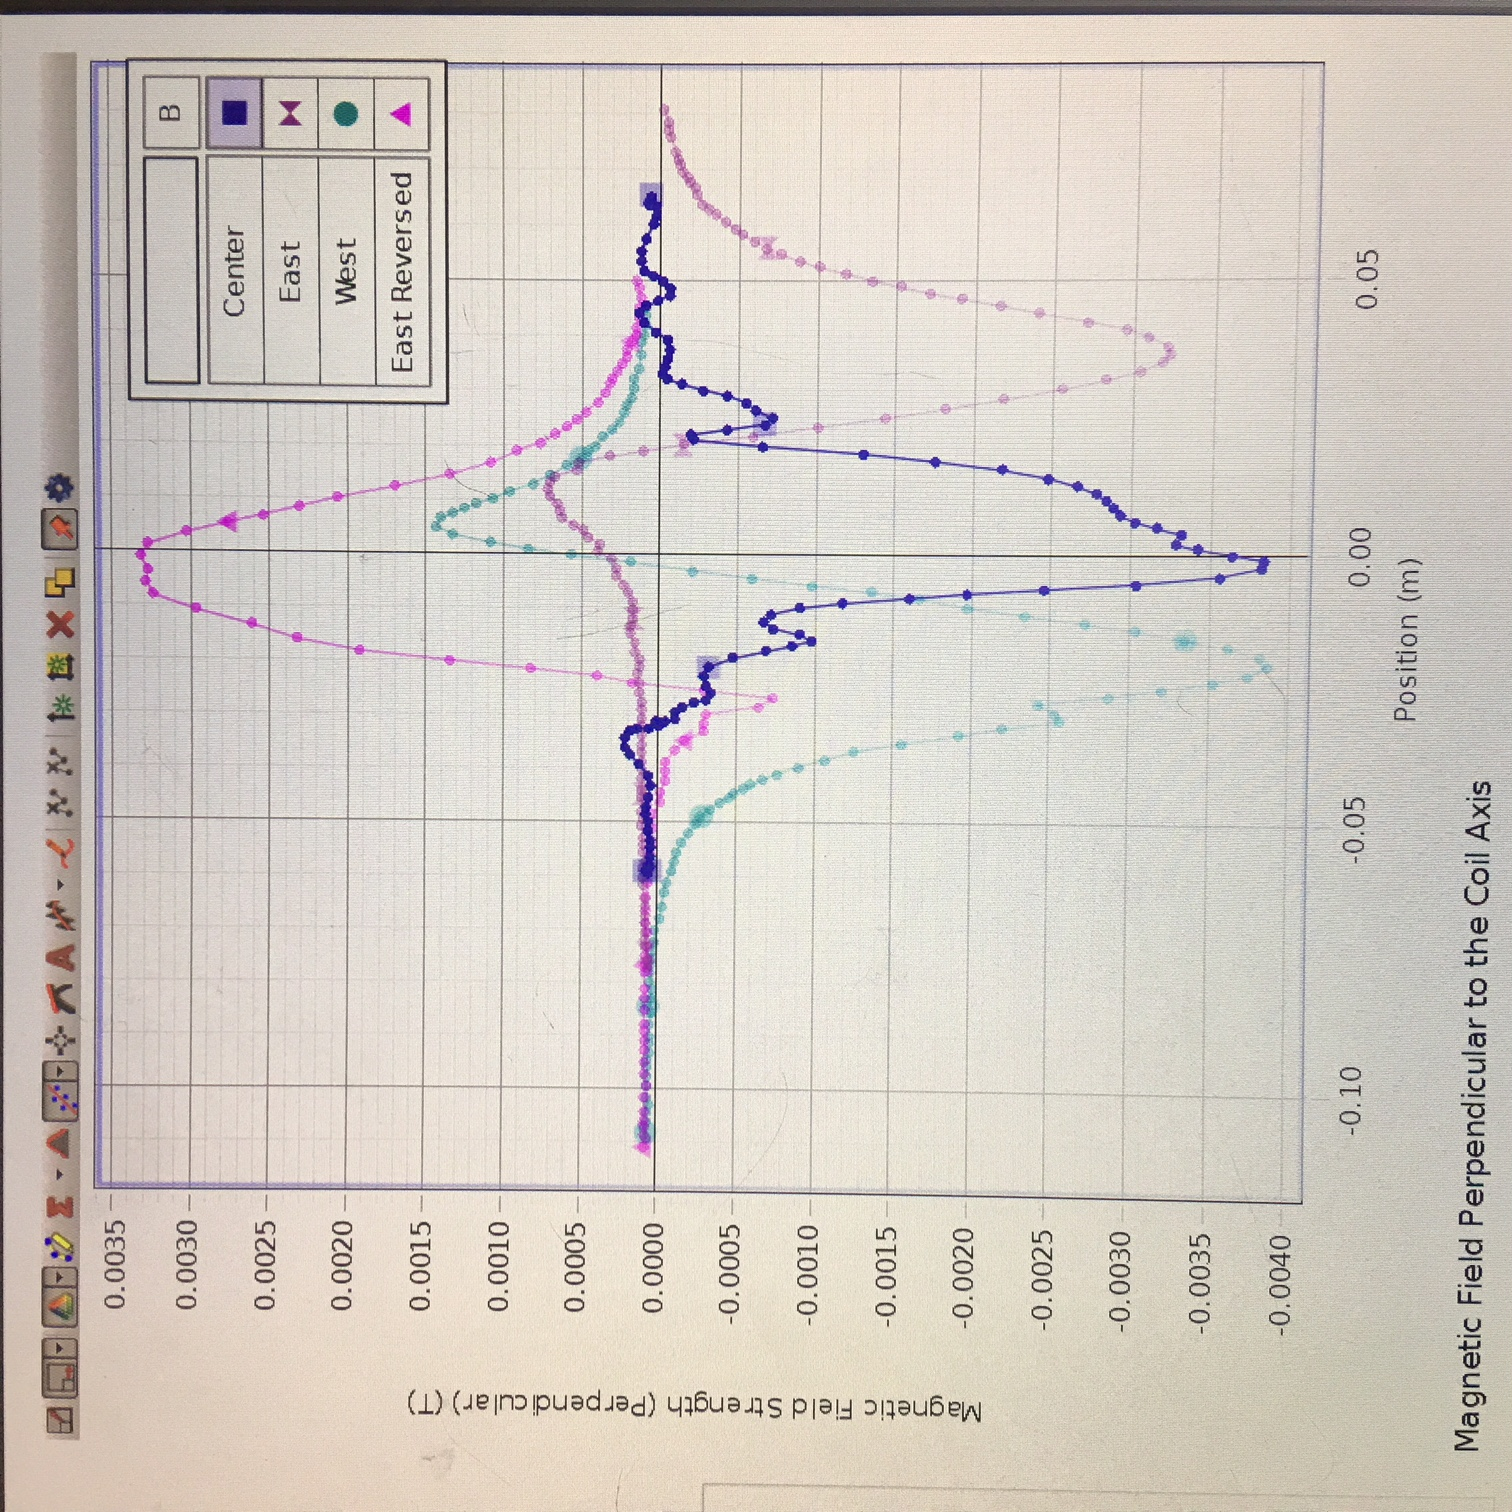
\includegraphics[width=.9\textwidth,angle=270]{radial.jpg}
    \end{minipage}

\end{minipage}
\pagebreak

%% discussion

\section*{Discussion of Results and Error Analysis}

In the first three runs, the current is very close in strength. This shows that the axial field is uniform in strength across the coil. Overall, our data indicates that the direction of the magnetic field generated by the coil points upward, indicating that the current runs counter-clockwise around the coil. This is supported by the construction of the circuit, in which the positive terminal of the signal generator is connected to the coil on the right side, and the negative terminal is connected to the left side of the coil.

\bigskip
The direction of the current is reversed when the terminals are switched, so it follows that the axial peak amplitude of the \textit{East, rev} run is negative while the others are positive. In that run, the current runs clockwise in the coil and the magnetic field points downward. This difference in current flow direction between the \textit{West} and \textit{East, rev.} runs (and similarly, the reversed polarity of the magnetic field between the two) explains the difference in the graphs of the radial field strength with respect to the position of the sensor probe.

\bigskip
The calculated bound values using Equations \ref{single_coil} and \ref{long_solenoid} were both higher than the measured axial peak amplitudes. The measured amplitudes were all closer to that of a short solenoid than to that of a long solenoid.

\bigskip
Due to the symmetry of the system, the radial component of the field should be zero. However, since we were measuring the magnetic field of the coil at its ends, the existence of a non-zero radial component shows the behavior of the magnetic field past the ends of the coil. Based on our data, it appears that the field, as represented by magnetic field lines, curves in toward the center of the coil as the lines enter the coil, and out away from the center of the coil as the lines leave the coil. This explains why the radial field in the \textit{East} and \textit{West} looks the way that it does.

\bigskip
The appearance of a non-zero radial component in the \textit{Center} run is due in large part to error. While removing the sensor probe from the center of the coil, we allowed the probe to move slightly in a direction perpendicular to the vertical axis of the coil. This introduced a source of experimental error, which does not necessarily show the existence of a non-zero radial component for that run.

%% conclusion

\section*{Conclusion}

We conclude that the magnetic field is aligned with the axis of the coil up until the ends of the coil, at which point the positive end of the field curves around and "re-enters" the coil at the negative end. We found the coil to behave more like a short solenoid than a long solenoid, with magnetic field strength less than that of either model.

\bigskip
Our failure to keep the sensor probe aligned with the axis of the coil introduced a non-zero radial component to the magnetic field and thus introduced a major source of error in several of the runs. Correcting this error would improve the accuracy of the results greatly; however, this is not an indication that the method used is inaccurate or imprecise.


%% done

\end{document}

%%% document above %%%